\subsection{Model Implementation}

\begin{figure}[h]
	\centering
    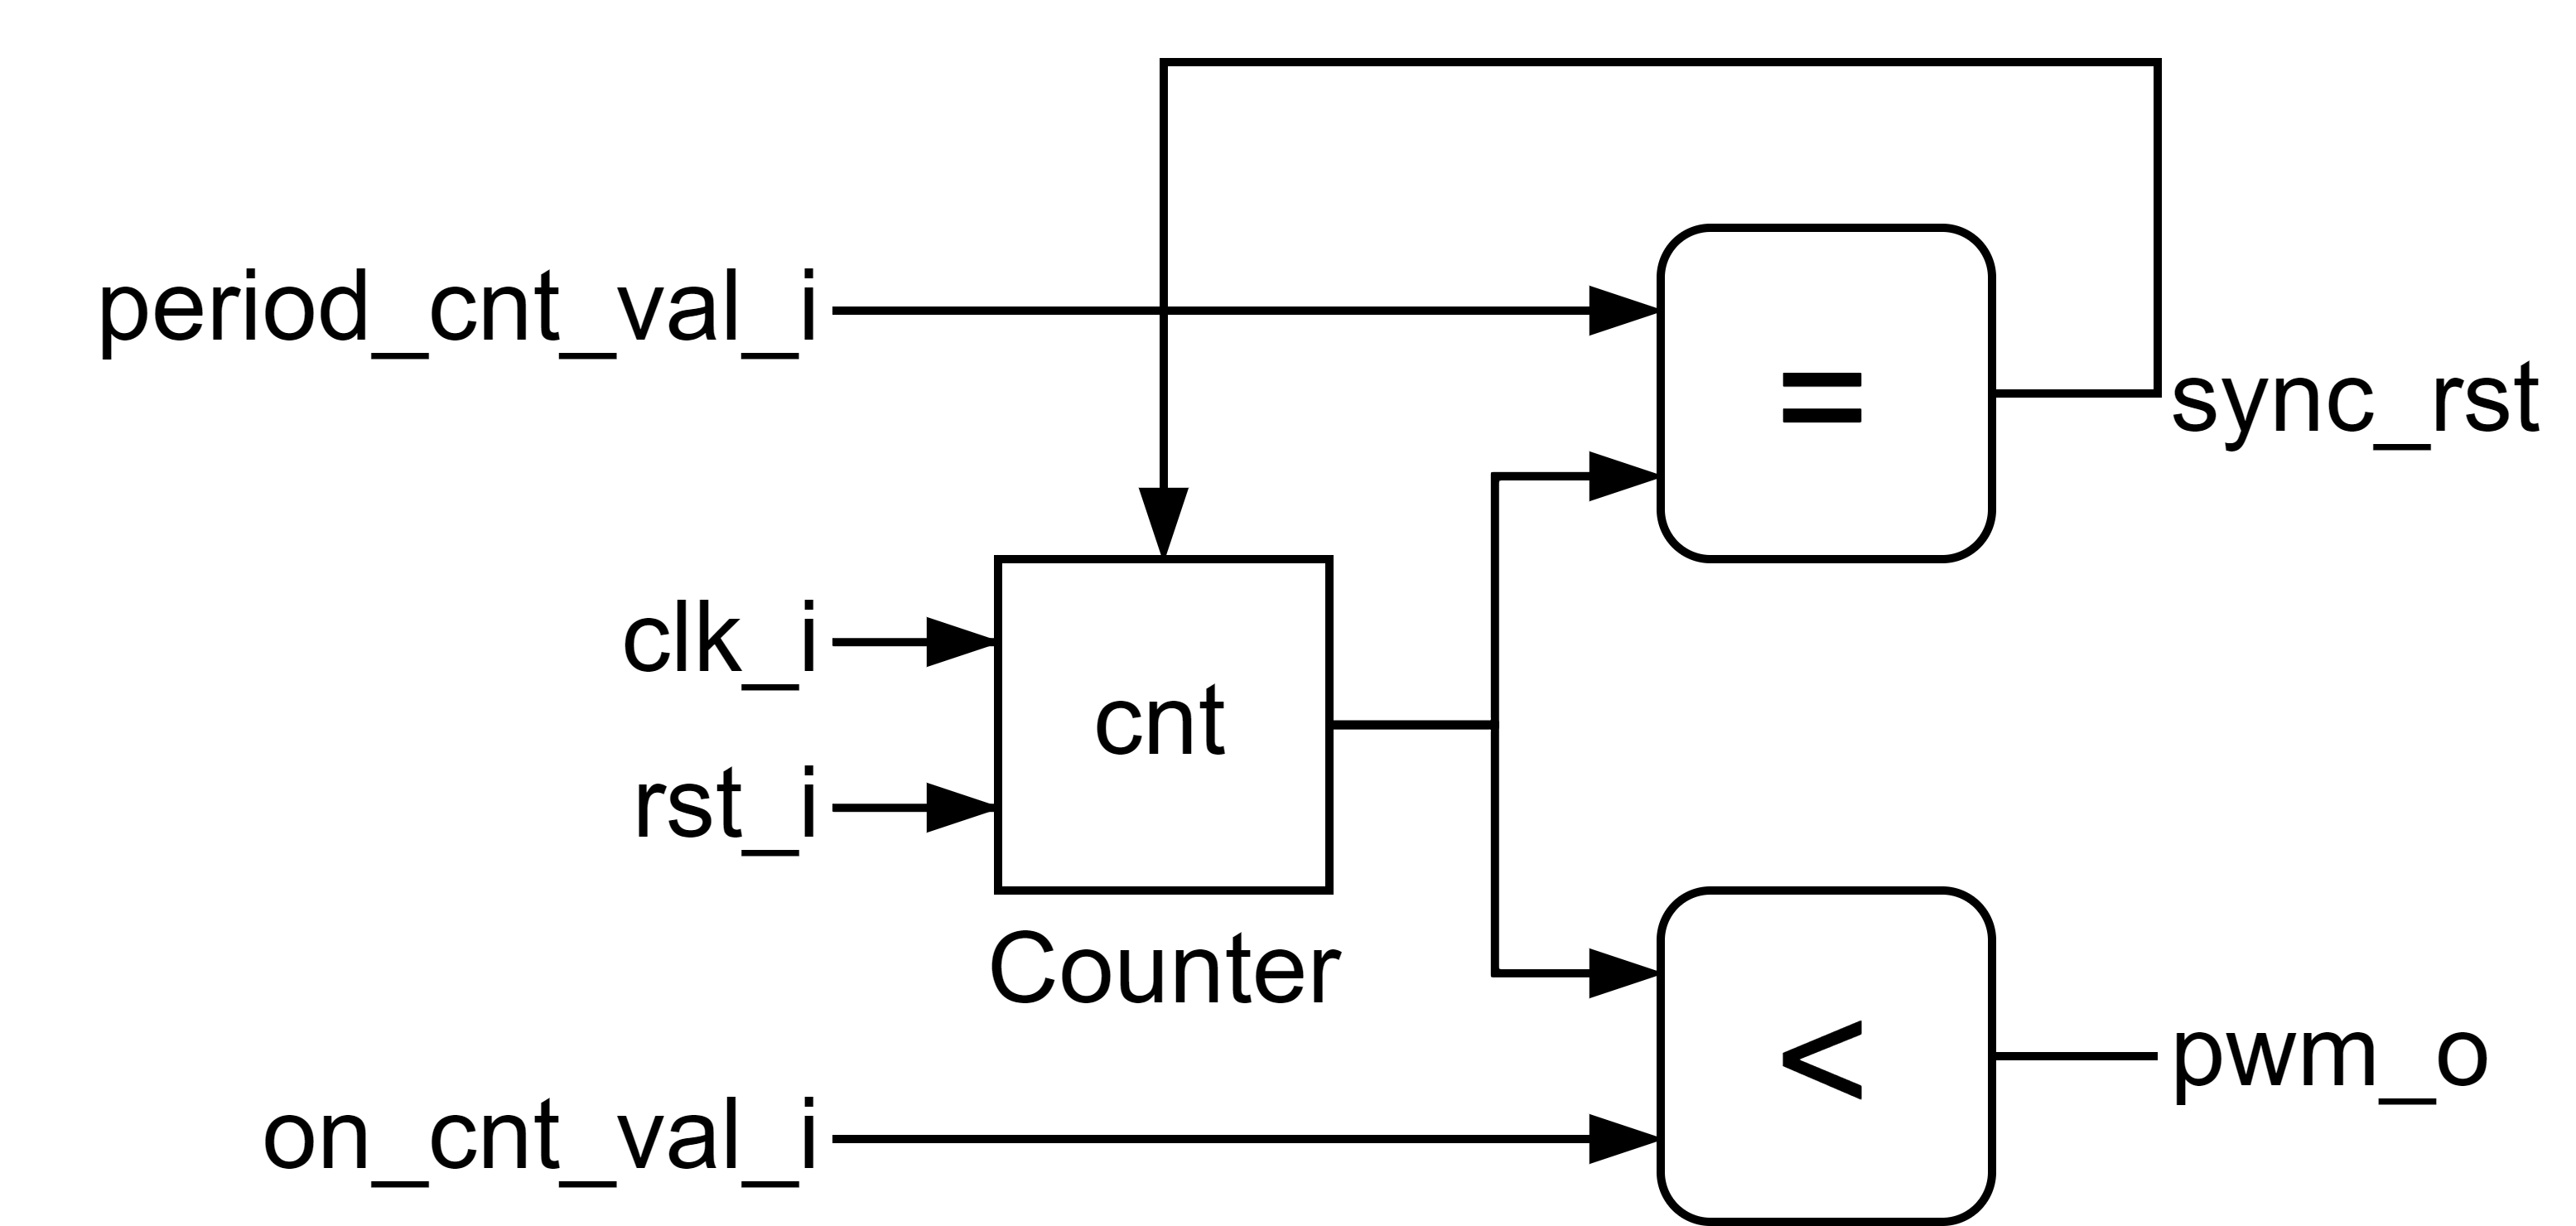
\includegraphics[width=0.6\linewidth]{images/PWM-Arch.png}
	\caption{PWM Architecture}
\end{figure}

The PWM generator uses a counter to count up to the specified period. When the
counter value is less than the duty cycle, the output signal is high and
otherwise low. The counter resets when it reaches the period value. As the
counter only consist of one register process as seen in EX02 and the PWM module
only adds combinatorics to the output, no state-machine is needed.

The \textit{counter} is reused from EX02 and is instantiated:

\lstinputlisting[
	caption={Counter process},
	label={lst:cnt},
	firstline=21,
	lastline=30,
]{../pwm_a.vhd}

\newpage

The ``<''-Block is implemented as following process:

\lstinputlisting[
	caption={PWM Output process},
	label={lst:pwm},
	firstline=32,
	lastline=32,
	numbers=none
]{../pwm_a.vhd}

The ``=''-Block is implemented as following process:

\lstinputlisting[
	caption={Counter Reset process},
	label={lst:rst},
	firstline=33,
	lastline=33,
	numbers=none
]{../pwm_a.vhd}

\subsection{Simulation}

Waveforms of various period and duty cycle values are shown below.

\begin{figure}[h]
    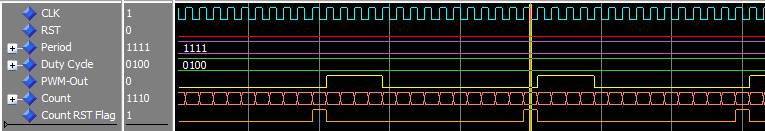
\includegraphics[width=\textwidth]{images/Sim1.png}
	\caption{Behaviour with Period 15 and Duty Cycle 4}
\end{figure}

\begin{figure}[h]
    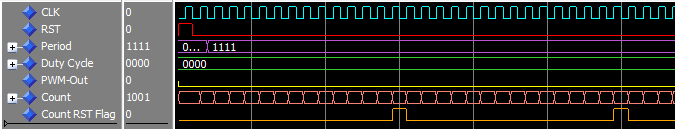
\includegraphics[width=\linewidth]{images/Sim2.png}
	\caption{Behaviour with Period 15 and Duty Cycle 8}
\end{figure}

\begin{figure}[h]	
    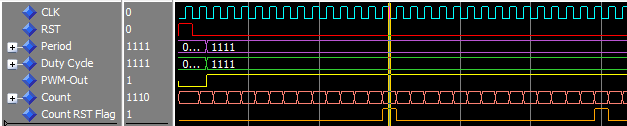
\includegraphics[width=\linewidth]{images/Sim3.png}
	\caption{Behaviour with Period 15 and Duty Cycle 15}
\end{figure}
